\chapterLabel{Terminology and Algorithm}

\sectionLabel{Winnow Algorithm}

\subsectionLabel{Basic Idea}

Put simply, \textit{Winnow} is a machine learning technique for discerning the
disjunction, (i.e.\ the \textbf{OR}ing function) from labelled examples.
Concretely, what this means is, given \(m\) labelled samples, each with a
vector of \(n\) Boolean features \(x = \{x_1, \ldots, x_n\}\), Winnow learns
which features to union to get the correct label.

Take the example of email spam filtering, on the basic level, we will take the
body of the many emails, and tokenize them into array of words, this will be
our features vector.

Each feature (word) is denoted by \(1\) if it exists in the example, \(0\) if
it doesn't.

\addcontentsline{lot}{table}{Example for \textit{Winnow Algorithm}}
\begin{tabularx}{\textwidth}{c c c c c c c c}
    \(x_1\)    & \(x_2\)   & \(x_3\)  & \(x_4\)    & \(x_5\) & \(\ldots\)               & \(x_n\)    & \(\text{spam (yes/no)}\)\\
    \(\$\$\$\) & \(100\%\) & \(free\) & \(viagra\) & \(the\) & \(weight\text{\ } loss\) & \(\ldots\) & \(f(x)\)\\
    \(0\)      & \(1\)     & \(0\)    & \(1\)      & \(0\)   & \(1\)                    & \(\ldots\) & \(?\)
\end{tabularx}

Now we can see the problem, the feature set can be very large, with many
features set to \(true\) (the \(for\) example occurs in almost every email) yet
the correct labelling depends only on a small subset of features \(r\).

\subsectionLabel{Working}

\addcontentsline{lot}{table}{Working of \textit{Winnow Algorithm}}
\begin{enumerate}
    \item Initialize the weights \(w_1 = w_2 = \ldots = w_n = 1\) on the \(n\)
    variables (features vector).
    \item Given an example \(x = \{x_1, \ldots, x_n\}\), output \(1\) if:\\
    \(\displaystyle\sum_{i=1}^{n} w_i\, x_i \geq \theta\)\\
    else output \(0\).\\
    \(\theta\) is a threshold value we set to our discretion.
    \item If the algorithm makes a mistake:
    \begin{enumerate}
        \item If it predicts \(0\) when \(f(x) = 1\), then for each \(x_i = 1\), increase the value of \(w_i\). (value was too low, promote contributing features)
        \item If it predicts \(1\) when \(f(x) = 0\), then for each \(x_i = 1\), decrease the value of \(w_i\). (value was too high, demote contributing features)
    \end{enumerate}
\end{enumerate}

Winnow gives us a mistake bound of \(O(r\, log(n))\). Where, \(r\) is the number
of relevant features and \(n\) is the total number of features.

\begin{figure}[h]
    \centering
    \caption{Flowchart of the algorithm}
    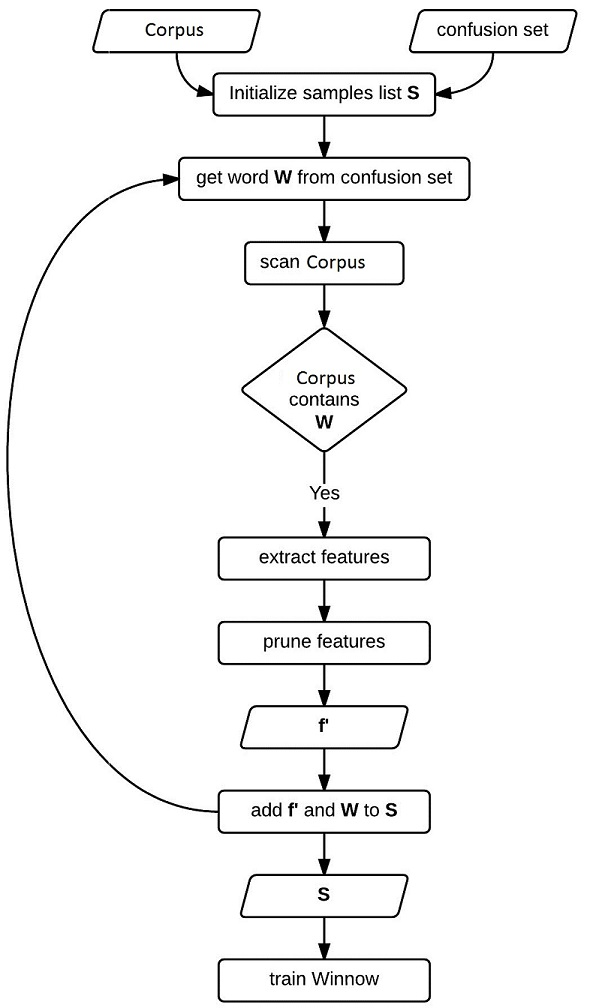
\includegraphics[height=165mm]{img/Flowchart.jpeg}
\end{figure}
\null\vfill
